% APORIA 2025
% For licence: see LICENSE

\documentclass[twoside]{book}

\title{Aporia 25}
\author{University of St Andrews Philosophy Society}
\date{2025}

% Paper size and margins
\usepackage[
    a4paper,
    outer=1.625in,
    inner=1.125in,
    top=1.5in,
    bottom=1.5in
]{geometry}
% Fonts
\usepackage{ebgaramond-maths}
\usepackage{amssymb}                    % Math symbols (e.g. therefore)
\usepackage{enumitem}                   % indenting next line of list
\usepackage[scale=0.78]{plex-mono}      % Monospace font
\usepackage[T1]{fontenc}                % T1 character encoding
\usepackage{microtype}
\usepackage{hanging}                    % For bibliographies
\usepackage{ragged2e}
% Columns
\usepackage{multicol}
% Include PDFs
\usepackage[final]{pdfpages}
% Links
\usepackage[anythingbreaks]{breakurl}
\usepackage[hyphens]{url}
\usepackage{hyperref}
\hypersetup{
    colorlinks,
    linkcolor={red!50!black},
    citecolor={blue!50!black},
    urlcolor={blue!80!black}
    }
\urlstyle{tt}
% Headers
\usepackage{fancyhdr}
% Headings
\usepackage[raggedright]{titlesec}
% for cftchapleader and cftdotsep in Table of Contents
\usepackage{tocloft}
% for WithSuffix
\usepackage{suffix}
% for list processing tools
\usepackage{etoolbox}

% Gap definitions
\def \hangingindent {3em}
\def \credgap {15pt}
\def \ackgap {10pt}
% Table of contents
%   depth = 0 ; only display article entries in ToC (not other
%   headings)
\setcounter{tocdepth}{0}
%   dots in the listing for chapters
\renewcommand{\cftchapleader}{\cftdotfill{\cftdotsep}}
% Heading styles
\renewcommand\thesection{\arabic{section}}

\titleformat{\chapter}[display]{\sffamily\LARGE\bfseries\raggedright}{}{0em}{}
\titlespacing*{\chapter}{0pt}{-50pt}{40pt}
\titleformat{\section}{\large\bfseries\raggedright}{{\sf\thesection}}{2em}{}
\titleformat{\subsection}{\bfseries}{{\sf\thesubsection}}{1.5em}{}
% Header style
\pagestyle{fancy}
\renewcommand{\chaptermark}[1]{%
\markboth{#1}{}}
\renewcommand{\headrulewidth}{0pt} % remove line under header
\fancyhead{}
\fancyhead[RO]{\small\sc\itshape\leftmark}
\fancyhead[LE]{\small\sc Aporia Vol. 25}
\fancyhead[RE]{\small\sc\itshape\leftmark}
\fancyhead[LO]{\small\sc Aporia Vol. 25}

% Define chapterauthor
\newcommand\chapterauthor[1]{\authortoc{#1}\printchapterauthor{#1}}
\WithSuffix\newcommand\chapterauthor*[1]{\printchapterauthor{#1}}
\makeatletter
\newcommand{\printchapterauthor}[1]{%
    {\parindent0pt\vspace*{-25pt}%
    \linespread{1.1}\large\scshape#1%
    \par\nobreak\vspace*{35pt}}
    \@afterheading%
}
\newcommand{\authortoc}[1]{%
    \addtocontents{toc}{\vskip-00pt}%
    \addtocontents{toc}{%
        \protect\contentsline{chapter}%
        {\hskip1.3em\mdseries\scshape\protect\normalsize#1}{}{}}
    \addtocontents{toc}{\vskip5pt}%
}
\makeatother
% Define acknowledgementlist
\makeatletter
\newcommand\acknowledgementlist[1]{%
    \forcsvlist{\acknowledgementlist@item}{#1}
}
\newcommand\acknowledgementlist@item[1]{
    \noindent#1%
    \par
    \vspace{\credgap}
}
\makeatother
% Define refsection
\def \refsection {\newpage\section*{Bibliography}}

% MAIN
\begin{document}
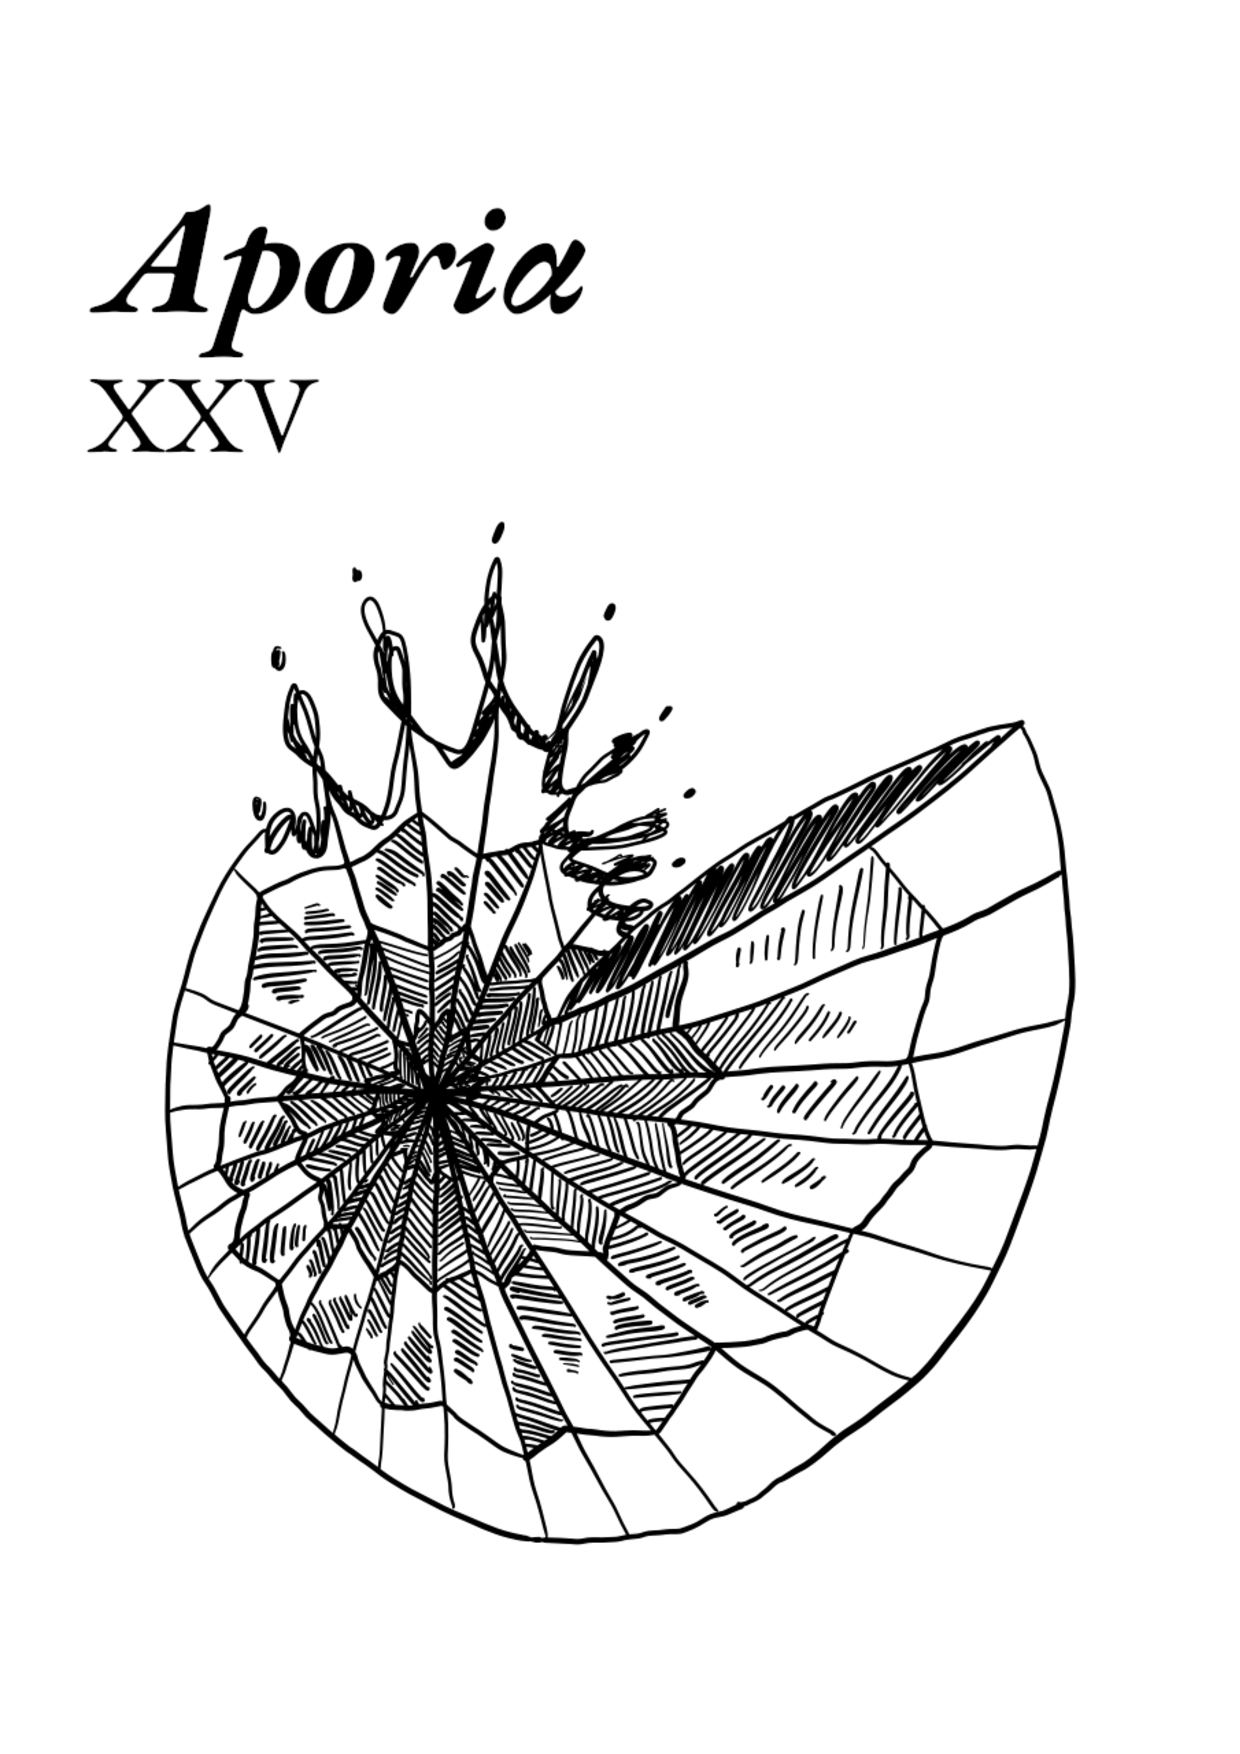
\includepdf{COVER.pdf}
\thispagestyle{empty}
\frontmatter
\begin{center}
    \vspace*{7cm}
    
    {\huge\textit{Aporia}}

        \vspace{3cm}
    \normalsize
    Undergraduate Journal of the St Andrews Philosophy Society

    \vspace{1cm}
    VOLUME XXV
\end{center}

\vfill 

\noindent \textit{Aporia} is funded by the University of St Andrews Philosophy
Society, which receives funds from the University of St Andrews
Department of Philosophy, the University of St Andrews Students’
Association, and independent benefactors.

\vspace*{\credgap}
\begin{center}
    \LARGE \sc Foreword
\end{center}

\vspace{\ackgap}\noindent
Congratulations to all those involved with \emph{Aporia} for reaching
the milestone of a twenty-fifth volume! I was a first-year undergraduate
when the first issue was released. I look back at that day fondly. We
celebrated with a wine reception in Edgecliffe (though, to be entirely
honest, we didn't need much of an occasion to indulge in some wine!),
and there were speeches from Vera Schoeller (the society president) and
Professor Sarah Broadie, who was always a vocal supporter of PhilSoc.

The journal has also published some fantastic work over the years,
including by authors who have gone on to be very successful professional
philosophers. The very first issue included pieces by Marcus Rossberg
and Philip Ebert (now professors at Connecticut and Stirling,
respectively) and a special contribution from Duncan Pritchard (now UC
Irvine). Later issues included Andreas Stokke (Uppsala), Fenner Tanswell
(Technical University Berlin), Steffen Koch (Bielefeld) and Michael
Hicks who is currently my colleague at the University of Glasgow. I was
a co-editor (with Kyle Mitchell) for volumes II and III. I was also
tasked with designing and formatting (which, unfortunately, was not my
forte). Since my time at the helm, I am pleased see that the high
quality of philosophy has continued, and the design quality has
significantly improved. The journal is now an extremely
professional-looking production, and something for all involved to be
proud of.

The St Andrews Philosophy Society will always hold a very dear place in
my heart. It was there that I got to know many people who are my friends
until this day. It is wonderful that the society is still going strong,
and that the journal continues to be a roaring success.

\vspace{\ackgap}\noindent
Dr Joe Slater

\noindent
Lecturer in Moral and Political Philosophy, University of Glasgow

\noindent
St Andrews Philosophy Society President (2011/12)

\vspace*{\credgap}
{\noindent\LARGE\sc Letter from the Editor}
\vspace{\credgap}

\vspace{\ackgap}\noindent
Dear Reader,

\vspace{\credgap}\noindent
It is with pleasure that I present the 25\textsuperscript{th} edition
of \emph{Aporia}, the undergraduate philosophy journal of St Andrews.
I hope it shall prove a stimulating and enjoyable read.

My particular thanks, firstly, to Joe Bradstreet, my deputy, who has
been a well-informed and clever editor, a diligent administrator, and
a pleasant balance to all my neuroticisms. My thanks also to Christina
Llandys Herre, who bravely shouldered much of the administrative
burden.  And I cannot fail to mention Mohit Agarwal, whose technical
prowess and willingness to take on tasks far beyond my capabilities
have been utterly invaluable. I am extremely grateful to the whole
editorial team for their dedication, expertise, and good humour; I
should have been quite at sea with many of the papers were it not for
their excellent work.

I am often teasingly asked about our readership; I think I may honestly
answer that the people who truly gain the most from \emph{Aporia} are
the editors and writers. From my editorship I have been exposed to areas
of philosophy untouched by my courses, learned more about the rights
(and perhaps more frequently wrongs) of academic writing than any
lecturer has taught me, and acquired the skill of working with a
relatively large and diverse team. For all the vexations of the
position, I am pleased to have had the opportunity of dipping my toe
into the murky waters of academic research and publishing.

It is a real triumph that \emph{Aporia} has survived 18 years of
disorganized philosophy students, incomprehensible technological
advancements, interrupted teaching, and unreliable funding. Let us hope
it shall long continue for the next generations of budding philosophers.

\vspace{\credgap}\noindent
Yours faithfully,

\vspace{\ackgap}\noindent
Kirsty Graham

\noindent
Editor-in-Chief, \emph{Aporia}

\vspace*{\credgap}
{\noindent\LARGE\sc Acknowledgements}

\vspace*{\fill}
\begin{multicols}{2}
{\noindent\Large\sc Editors}
\vspace{\credgap}

\acknowledgementlist{
    Aliza Ashraf,
    Beth Cook,
    Maria de Feo,
    Ella Johnston,
    Hanaa Khan,
    Zack Ledesma,
    Christina Landys Herre,
    Nawal Mirza,
    Claire Mizrahi,
    Phoebe Ray,
    Nathalie Rogers,
    Rosa Velasco Saavedra,
    Jacob Walchuk,
    Hoochang Yi
}
\columnbreak
\vspace*{\fill}
\acknowledgementlist{
Kirsty Graham\newline\emph{Editor-in-Chief},
Joe Bradstreet\newline\emph{Deputy Editor-in-Chief},
Mohit Argawal\newline\emph{Technical Officer}
}
\vspace*{\fill}
\end{multicols}
\vspace*{\fill}

\tableofcontents
\clearpage
\thispagestyle{empty}

\mainmatter

\chapter{Selfish Comparative Optimism: A Rejoinder to Nagasawa's \emph{Problem of Evil for Atheists}}
\chaptermark{Selfish Comparative Optimism}
\chapterauthor{Wilson Sugeng,
\textit{University of St Andrews}}


% Makes the section headings be formatted so it does `Section 1:', instead of just '1'
\renewcommand*{\thesection}{Section~\arabic{section}:} 
% \thesubsection might use \thesection, therefore it is also redefined
\renewcommand*{\thesubsection}{\arabic{section}.\arabic{subsection}}


\begin{quote}
Yujin Nagasawa's problem of systemic evil (POSE) argues that systemic
evils like natural selection pose a greater challenge to
atheism/non-theism than to theism, as they conflict with ``modest
optimism'': the view that the world is fundamentally ``not bad.''
Nagasawa suggests theism resolves this by appealing to a heavenly bliss,
offsetting natural evils, a strategy unavailable to
atheists/non-theists. However, I argue that atheists/non-theists are
better equipped to address POSE because they are not constrained by the
theistic commitment to a categorically good world.

In Section $1$, I critique two theistic approaches to POSE. Extreme
optimism defends the actual world as the best possible one, requiring
problematic justifications such as free-will and ``only-way'' theodicies
to explain systemic evils as necessary. Neutral optimism, while allowing
for multiple good worlds, still struggles to reconcile systemic evils
with a benevolent God, merely shifting the problem to other possible
worlds.

In Section $2$, I explore how atheists/non-theists can bypass POSE. They
can adopt personal, rather than cosmic, optimism, valuing their own
existence without affirming the world's overall goodness. Alternatively,
they can embrace comparative optimism, viewing existence as better than
non-existence without attributing intrinsic value to natural processes
like evolution. These flexible approaches free non-theists from the
philosophical burdens tied to systemic evils.

In Section $3$, I argue that even if POSE persists, atheists/non-theists
can ``borrow'' theists' theodicies without committing to their
metaphysical assumptions. By adopting naturalistic or subjective
frameworks, non-theists can justify their modest optimism without the
theological constraints imposed by theism. This demonstrates that POSE
ultimately challenges theistic frameworks more than atheistic ones.
\end{quote}

\vspace{\credgap}

\section*{Introduction}

In \emph{The Problem of Evil for Atheists,} Yujin Nagasawa develops a
problem of systemic evil (POSE) that he claims challenges both
atheists/non-theists and theists alike.\footnote{When I say, ``God'' and
  ``Theism'' in this paper, I assume an omniscient, omnipotent, and
  omnibenevolent singular/simple creator.} He identifies a tension
between two widely held theses: 

\begin{enumerate}[leftmargin=42]
\def\labelenumi{(\arabic{enumi})}
\item
  Systemic evil: The process of natural selection necessitates
  significant suffering and pain for countless sentient animals.
\item
  Modest optimism: Overall and fundamentally, the environment in which
  we exist is not bad.\footnote{Yujin Nagasawa, \emph{The Problem of
    Evil for Atheists} (Oxford University Press, 2024), 133, 140.}
\end{enumerate}

\noindent While theists naturally affirm modest optimism due to their belief in a
benevolent creator God, Nagasawa observes that atheists/non-theists are
also generally grateful for their existence.\footnote{Nagasawa,
  \emph{The Problem of Evil for Atheists}, 161.} For instance, popular
atheist Richard Dawkins suggests that contemplation of the law-like
evolutionary processes behind our existence puts us ``in a position to
give thanks for our luck in being here''---not a gratitude directed
towards any agent or being, but rather a ``gratitude in a
vacuum.''\footnote{Richard Dawkins, ``The Greatest Show on Earth
  Live'' (lecture, University of Auckland, Auckland, New Zealand, 13
  March 2010).} Nagasawa sees this as inconsistent: expressing
existential gratitude without acknowledging the systemic evils
underpinning it implies a tacit endorsement of these evils.

To illustrate this tension, Nagasawa adapts Janna Thompson's apology
paradox, which holds that regretting an unjust historical event can be
problematic if one's existence depends on that event. For example, a Jew
whose grandparents met during the Holocaust faces a paradox: to regret
the Holocaust may seem to imply regretting her own existence.\footnote{Janna
  Thompson, ``The Apology Paradox,'' \emph{The Philosophical Quarterly}
  50\emph{,} No. 201 (2000): 471.} Thompson resolves this by
distinguishing between regretting \emph{how} one came to exist and
\emph{that} one exists---the Jew can regret \emph{how} her grandparents
met, without regretting \emph{that} they met at all.\footnote{Janna
  Thompson, ``The Apology Paradox,'' \emph{The Philosophical Quarterly}
  50\emph{,} No. 201 (2000): 475.} Applied to POSE, this seems to suggest that one can regret the
mechanisms of natural selection without regretting the outcome of our
existence.

However, Nagasawa argues that this resolution fails in the context of
POSE. Unlike historical events, natural selection is not a contingent
circumstance but a fundamental feature of the natural world.\footnote{Nagasawa,
  \emph{The Problem of Evil for Atheists}, 167.} To reject it is not to
regret a particular pathway to existence, but to undermine the very
conditions that make existence possible. That is, there is no possible
world where natural selection does not govern nature and beings like us
still exist.

Theists, Nagasawa argues, are better positioned to defend modest
optimism, drawing on ``heavenly bliss'' theodicies that justify or
outweigh earthly suffering with the promise of an afterlife. These come
in two forms: (1) as a deferred justification, where evolution is
acceptable because it leads to eternal reward, and (2) as a utilitarian
offset, where infinite heavenly bliss outweighs finite worldly
suffering. Because atheists cannot appeal to such concepts, POSE, he
claims, presents a more serious problem for atheists.

Contrary to Nagasawa, I argue that atheists and non-theists are better
positioned to address POSE because they are not constrained by the
theistic requirement to see the world as overall categorically good. To
support this claim, I first critique two theistic attempts at resolving
systemic evil, namely extreme and neutral optimism, illustrating their
shortcomings. Subsequently, I explore how atheists/non-theists might
effectively sidestep POSE by adopting personal rather than cosmic
optimism, or by embracing a comparative optimism which sees existence as
preferable to non-existence without categorically endorsing the systems
that facilitated it. Finally, I turn Nagasawa's borrowing argument
around to propose that, even if POSE remains challenging,
atheists/non-theists can strategically adopt theistic theodicies without
their accompanying metaphysical assumptions, thereby reducing POSE's
impact and revealing it to be ultimately a greater challenge for
theistic frameworks than for atheistic or non-theistic ones.

\section{Two Theist Modest Optimists}
\subsection{Extreme optimism}

The first theist modest optimists---extreme optimists---claim that
because God actualised the best among all possible worlds, systemic evil
must necessarily exist in all good worlds. Although Gottfried Wilhelm
Leibniz does not himself discuss systemic evil and predates evolution,
his \emph{Theodicy} (1710) presents a system where given God's
omnibenevolence and omniscience---if a possible world is better than the
actual, then God would either not be good enough to desire the best for
the world, or ignorant in not knowing which world is the
best.\footnote{G. W. Leibniz, \emph{Theodicy,} edited by Austin Farrer,
  translated by E. M. Huggard (Open Court Publishing Company, 1985),
  249.}

As an implication, extreme optimists must affirm Nagasawa's claim that
no possible world exists in which natural selection does not govern
nature; for if God is necessary, then no other world is possible.
Natural selection must therefore serve an instrumental role in the
world's goodness. Building on this system, Austin Farrer argues that the
removal of any such purported evil systems will undermine God's
mechanism for bringing about the best world. The goodness of a physical
system, for instance, inherently includes the potential for mutual
interference, leading to evils like predation. Without this
interference---if this world were a ``magically self-arranged garden''
free of competition for space or resources---physicality itself ceases
to exist.\footnote{Austin Farrer, \emph{Love Almighty and Ills
  Unlimited} (Collins, 1962), 53-54.} Removing such systems would
be akin to relieving an animal's pain ``by the removal of its nervous
system; that is to say, of its animality.''\footnote{Austin Farrer, \emph{Love Almighty and Ills Unlimited} (Collins, 1962), 51.}
Regretting natural selection thus implicitly challenges God's
rationality and goodness in creating us as physical beings rather than
spiritual entities.\footnote{Austin Farrer, \emph{Love Almighty and Ills
  Unlimited} (Collins, 1962), 67.}

An immediate difficulty with extreme optimism is that claiming this
world to be the best possible one is hard to reconcile with the presence
of seemingly avoidable evils observed throughout nature. This tension is
captured ironically in the eponymous character of Voltaire's
\emph{Candide} (1759) who insists that this is the best possible world
as he faces a world plagued with wars, earthquakes, and
slavery.\footnote{Nagasawa, \emph{The Problem of Evil for Atheists,}
  129.} Or when Darwin questions why God permitted the creation of the
Ichneumonidae who brutally feeds inside the living bodies of
caterpillars.\footnote{Charles Darwin, ``22 May 1860 Letter to Asa
  Gray,'' Darwin Correspondence Project, accessed on 5 December 2024,
  https://www.darwinproject.ac.uk/letter/DCP-LETT-2814.xml.} This
presents a major challenge: extreme optimism struggles to align with
observable, avoidable evils unless it denies these empirical
observations---as some Creationists do---or reinterprets such systemic
evils as necessary.\footnote{Paul Prescott, ``The Secular Problem of
  Evil: An Essay in Analytic Existentialism,'' \emph{Religious Studies}
  57 (2021): 102.}

Granting natural selection's empirical truth, theists generally present
two kinds of theodicies for \emph{why} God actualised natural selection.
Firstly, theists have adapted the free-will theodicy to address some
non-agential non-human suffering. In traditional free-will theodicies,
God permits agents the capacity to choose evil over good as the goodness
of human agency outweighs the risks of their choosing evil. In one
adaptation, Richard Swinburne argues that animal pain and suffering
exists as examples of evil actions humans can inflict on each other.
Predation therefore exists as an educational tool for humans to observe
and understand how to commit evil, thereby enabling their capacity for
moral choice.\footnote{Richard Swinburne, ``Natural Evil,''
  \emph{American Philosophical Quarterly} 15\emph{,} No. 4 (1978): 299.}

Secondly, theists have adapted a variation of the soul-making theodicy
known as the ``only-way'' theodicy, arguing that certain natural goods
can only develop through natural selection. Holmes Rolston observes that
the predator-prey cycle is instrumental to the beautiful diversity of
animals, where ``The cougar's fang has carved the limbs of the
fleet-footed deer, and vice versa.''\footnote{Holmes Rolston III,
  \emph{Science and Religion: A Critical Survey} (London: Templeton
  Foundation press, 2006), 134.} While Young-Earth Creationism may have
created this diversity instantaneously, Christopher Southgate argues
that natural selection is the only way creatures can develop into
biological ``selves'' with their own interests and
behaviours.\footnote{Southgate, \emph{The Groaning of Creation}, 58.}
This offsets any evolutionary evils for it culminates into complex
``selves'' that conform to God's image.\footnote{Southgate, \emph{The Groaning of Creation}, 72.} This
``selving'' must come independently, for Peter van Inwagen argues that
an irregular world is a defect: God who constantly intervenes and
violates his own laws is either a irrational or evil.\footnote{Peter van
  Inwagen, ``The Problem of Evil, the Problem of Air, and the Problem of
  Silence,'' \emph{Philosophical Perspectives} 5 (1991): 143-45.} So,
common to both free-will and ``only-way'' theodicies is a notion that
some ultimate good offsets the evils of natural selection as an
instrument.

However, these two theodicies only defer the problem of evil to another
system underlying the challenged system. For instance, free-will
theodicies must still address Pierre Bayle's objection: If God's
omniscience foresees that giving humanity free will inevitably results
in unrighteousness, then God is either reckless or cruel to ``gift''
humanity agency, knowing it would lead to their harm and judgment under
his wrath.\footnote{Pierre Bayle, \emph{Historical and Critical
  Dictionary: Selections,} translated by Richard H. Popkin and Craig
  Brush (Hackett, 1991), 177.} Echoing Bayle, Robert John Russell
questions, ``Why did God choose to create \emph{this} universe with
\emph{these} laws of physics knowing that they would not only make
Darwinian evolution unavoidable, and with it the sweep of natural evil
in the biological realm?''.\footnote{Robert John Russell, ``Natural
  Theodicy in an Evolutionary Context,'' in \emph{Cosmology: From Alpha
  to Omega} (Fortress Press, 2008), 259.} It appears, then, that extreme
optimism is burdened with regressive manifestations of the problem of
evil.

In sum, while extreme optimists attempt to reconcile systemic evil with
the claim that this is the best possible world through the use of
free-will and ``only-way'' theodicies, such strategies ultimately defer
rather than resolve the problem. Faced with empirical evidence of
seemingly gratuitous suffering, they must either deny these realities or
accept increasingly speculative theological explanations. While extreme
optimism may appeal to the heavenly bliss defence, it still does not
explain \emph{why} natural selection is the best possible means towards
that end without returning to this regress or begging the question. As
such, extreme optimism appears ill-equipped to resolve the tension
Nagasawa identifies between systemic evil and modest optimism. So,
theists must either concede that natural selection is not the best
necessary instrument in the best possible world, or following Bayle and
Russell accept the former's pessimism or latter's ``agnostic cosmic
theodicy'' in accepting that POSE cannot be answered.\footnote{Robert John Russell, ``Natural Theodicy in an Evolutionary Context,'' in \emph{Cosmology: From Alpha
  to Omega} (Fortress Press, 2008), 255.}


\subsection{Neutral optimism}


The second theist modest optimists, the neutral optimists, reject that
the actual world is necessarily the best, but rather affirms that God
actualised one of many possible overall good worlds. For instance,
Robert Merrihew Adams argues that extreme optimism inappropriately
imposes a utilitarian standard of moral goodness to God's
omnibenevolence. Instead, he argues that traditional Judeo-Christian
ethics account for God's goodness in terms of his grace---an inclination
to love that is not based on the merit of the one being
loved.\footnote{Robert Merrihew Adams, ``Must God Create the Best?'',
  \emph{Philosophical Review} 81 (1972): 324.} Indeed, core to Abrahamic
monotheism is an affirmation of God's aseity, his self-sufficiency and
independence from any external cause or necessity. \footnote{Ian A.
  McFarland, \emph{From Nothing: A Theology of Creation} (Westminster
  John Knox Press, 2014), 61.} If God were obligated to create the best
possible world in order to express his power or love, then his
omnipotence and omnibenevolence would become contingent on something
external---namely, the existence of that world---thereby undermining his
aseity. It follows, therefore, that a being who never exists is not
wronged by not being created, since existence itself is not owed to any
potential being.\footnote{Adams, ``Must God Create the Best? 319-20.}
Furthermore, beings in the actual but not best world have no right to
complain, lest they express an unmerited claim for special treatment or
violate modest optimism.\footnote{Adams, ``Must God Create the Best? 319-20.} God's omnibenevolence,
therefore, does not demand that he create the best world possible.

As an implication, neutral optimists can entertain that there is a
possible world without natural selection where we exist. However, two
considerations may constrain this possibility. Firstly, this possible
world must be logically coherent. Thomas Morris argues that if God's
omnipotence is committed to what is logically and semantically possible,
God becomes a ``delimiter of possibilities.''\footnote{Thomas V. Morris,
  ``The Necessity of God's Goodness,'' \emph{New Scholasticism} 59
  (1985): 425.} That is, as God's existence is necessary in all possible
worlds, those worlds must reflect his omnipotence by being logically
coherent and his omnibenevolence by being overall good. This means that
if a world without natural selection either fails to be logically
coherent or cannot sustain overall goodness without introducing other
systemic evils, it may not be a genuine possibility after all. Secondly,
this limitation implies that a possible world without natural selection
where we exist is not necessarily better or worse than the actual world.
It could very well be that following the ``only-way'' theodicies, the
goodness of true biological selves must necessarily come through natural
selection and that this outweighs the evil of natural selection.
Regardless, the neutral optimist is distinct in that they can be
grateful for their existence without necessarily implying that natural
selection is instrumentally good.

One obvious challenge against neutral optimism is its shifting
definition of God's omnibenevolence may not be intuitively satisfying.
For instance, Adams's definition of God's ``grace'', which does not
require universal benevolence to all creatures, may only be satisfactory
to some Calvinists or those within certain theological traditions. While
this conception asserts that natural selection does not need to be
justified as instrumentally good, the reality and impact of systemic
evil make it difficult for suffering beings to reconcile that God's
omnibenevolence does not require him to show grace to them, in tension
with their own intuitions about what it means to be loving. However, as
this critique may hold less weight for those aligned with certain
Calvinist doctrines, where such a conception of grace is more readily
accepted, it will be set aside as a doctrinal matter.

A more universal challenge is that even if a neutral optimist can
maintain modest optimism about their existence while affirming systemic
evil through yearning for another possible world, logical constraints on
such worlds mean that regretting the evils of the actual world may
require relinquishing goods unique to its constitution. For example,
recalling Swinburne's free-will theodicy, a possible world without
natural selection might lead to it not having human agency. Similarly,
recalling Southgate's ``only-way'' theodicy, a world without natural
selection could lack independent selves. If the existence of goods like
human agency or autonomous selves carry significant moral weight, then
removing the conditions that produce them (i.e., natural selection) may
render the alternative world no longer overall good---and thus not
genuinely possible. At best, such possible worlds without natural
selection might not involve a loss of goods significant enough to
undermine modest optimism. At worst, the trade-offs could introduce
greater problems of evil. A creationist world, for instance, implies
that God played a direct role in designing cruel beings like the
Ichneumonidae than if they developed independently through evolution.

Comparing extreme and neutral theistic optimism, both conceptions of
modest optimism requires that the world is overall good. This is because
evidence of systemic evils must be outweighed by some other goodness or
burdened with a theodicy. This, however, is not a requirement for
atheist/non-theist optimism.

\section{Two atheist/non-theist modest optimists}
\subsection{Personal optimism}

The first atheist/non-theist modest optimist approach argues that the
scope of existential gratitude can be limited to the personal level
without axiologically considering the world as an aggregate. While
Dawkins expresses his gratitude for existing despite unfavourable odds,
he regrets that, ``Nature is red in tooth and claw. But I don't want to
live in that kind of a world. I want to change the world in which I live
in such a way that natural selection no longer applies.''\footnote{Frank
  Miele, ``Darwin's Dangerous Disciple: An Interview with Richard
  Dawkins,'' \emph{The Skeptic}, 27 October 2010,
  \url{https://www.skeptic.com/eskeptic/10-10-27/}.} However, we can
resolve Dawkins' apparent disjunct by affirming \emph{personal}
existential optimism directed at one's own existence while rejecting
\emph{cosmic} existential optimism that the world is overall good. This
is not methodologically novel; Asha Lancaster-Thomas observes that even
within individuals' lifetimes, we are grateful for some parts of our
lives, but not parts characterised by pain and suffering such as a
painful chronic illness.\footnote{Asha Lancaster-Thomas, ``Can Heaven
  Justify Horrendous Moral Evils? A Postmortem Autopsy,''
  \emph{Religions} 14, No. 296 (2023): 6.}

An implication of personal, but not cosmic, optimism is that their
existential gratitude does not need to consider the axiology of natural
selection. One could remain axiologically agnostic towards the
instruments of their existence, while valuing the goodness of their
personal existence. Guy Kahane emphasises this distinction by arguing
that even if natural selection is a causally fundamental instrument to
our existence, it is axiologically irrelevant as instrumental value
alone does not add any overall value to the world.\footnote{Guy Kahane,
  ``Optimism without theism? Nagasawa on Atheism, Evolution, and Evil,''
  \emph{Religious Studies} 58 (2022): 706.} Under this conception, one
could even be cosmically pessimistic but still be optimistic about their
personal life as they experience it. Modest optimism is thus
reinterpreted to affirm attitudinal optimism, that we are grateful to
exist in this world; but not axiological optimism, that the world is
overall good.\footnote{Guy Kahane, ``Optimism without theism? Nagasawa on Atheism, Evolution, and Evil,'' \emph{Religious Studies} 58 (2022): 702.}

However, after disregarding pessimism, personal optimism appears
empirically challenged as most personal optimists are often implicitly
also cosmic optimists. Responding to Kahane, Nagasawa grants that
personal optimism does not necessarily entail cosmic optimism. However,
he argues that this reformulation of modest optimism changes the target
of POSE, which defines modest optimism as affirming both attitudinal and
axiological optimism.\footnote{Nagasawa, \emph{The Problem of Evil for
  Atheists,} 184.} For he argues that rational personal optimists who
procreate implicitly believe that the world they are bringing their
child into is overall a good place.\footnote{Nagasawa, \emph{The Problem of Evil for
  Atheists,} 184.} The personal, but
not cosmic, reformulation of modest optimism, therefore, seemingly
misses the original target of POSE and is only applicable to a minority
of anti-natalist pessimists like David Benatar.

Responding to this, Nagasawa's formulation of modest optimism is already
limited to the scope of``the environment in which we exist.'' The
specific environment of individual experiences does not necessarily
include the predation experienced by other preyed beings. Indeed, this
does not preclude the modest optimist from being selfish for bringing a
child into the world. Or disregarding the pains of the world, a
personally optimistic individual can choose to be ignorant of the
world's plights by never contributing to charitable causes to use the
money to instead maximise personal pleasures. It is not evident,
therefore, that most personal optimists must also be cosmic optimists.

\subsection{Comparative optimism}

The second atheist/non-theist modest optimist approach argues that
modest optimism only views the world as \emph{comparatively} good, but
not necessarily \emph{categorically} good. That is, the world must only
be \emph{comparatively} better than non-existence, rather than
positively good. This distinction is significant, as Nagasawa's
comparative argument for theism seems to present the axiology of the
world in binary categorical terms. Theism's appeal to a heavenly bliss
allows for a world with more goodness rather than evil.\footnote{Nagasawa, \emph{The Problem of Evil for Atheists,} 171.} But because atheists/non-theists are not committed to affirming
an omnibenevolent God, Kahane argues that they are not obliged to claim
that their existence is categorically good, or that the world contains
more goodness than evil. Indeed, even under Leibniz's extreme optimism,
the world is not necessarily categorically good, just that it is
comparatively the best of all possible worlds.\footnote{Kahane,
  ``Optimism Without Theism,'' 713.}

An implication of a comparatively better, but not categorically good,
optimism is that natural selection does not have to be categorically
good. Assuming that existence in itself is a good greater than all kinds
of non-existence, an actual world with systemic evil is better than any
unactualised world. So, modest optimism's ``not bad'' is equated to
being comparatively better than non-existence. Opposing theism's appeal
to the supernatural, this essentially lowers the requirement for modest
optimism.

One major challenge is that this comparative-goodness version of modest
optimism closely borders on pessimism, and therefore demands an account
of why existence, despite systemic evils, is fundamentally and overall
better than non-existence. The pessimist Benatar, for instance, argues
that the absence of pain is always good, even if no one benefits,
whereas the absence of pleasure is only bad if someone is deprived by
it. This asymmetry supports his claim that existence, with its
inevitable suffering, may be worse than non-existence, which guarantees
goodness with no badness.\footnote{David Benatar, \emph{Better Never to
  Have Been: The Harm of Coming into Existence} (Oxford University
  Press, 2006), 30.}

Responding to Benatar, the optimist can follow Thaddeus Metz's argument
against Benatar's claim that the absence of pain is good, describing the
absence of pain as \emph{not bad} rather than \emph{good.}\footnote{Thaddeus
  Metz, ``Are Lives Worth Creating?'', \emph{Philosophical Papers} 40,
  No. 2 (2011): 241-45} Otherwise, the atheist/non-theist modest
optimist can simply appeal to the previously-discussed personal, rather
than cosmic, optimism. All modest optimism demands is that according to
myself, it is better for me to exist than for me not to exist. Indeed,
Benetar seems to grant this notion, as he distinguishes a present-tense
``life worth continuing'' and future-tense ``life worth
starting.''\footnote{Benatar, \emph{Better Never to Have Been,} 22-23.}
Personal optimists often experience instances where the goods of
actualised pleasure outweigh the evils of pain, resulting in a net
utility that makes existence preferable to non-existence. So, unless one
is personally pessimistic, there is nothing paradoxical about claiming
one's personal life is better to exist than not exist.

Combining these two approaches, the atheist/non-theist, can commit to a
personal and comparative form of modest optimism that still accounts for
the categorically systemic evil of the cosmos. Unlike theistic extreme
optimism's commitment to the instrumental value of natural selection as
a part of God's providence, personal optimists can simply remain
agnostic about natural systems' axiological value. But while theistic
neutral optimists can adopt a similar approach to the
atheism/non-theism's comparative (not categorical) goodness, they remain
committed to both that possible worlds must overall be good, and that
God's creative ability is bound to logical laws, so that the possible
worlds they yearn for must necessarily contain some other kind of
systemic evil that requires a theodicy . The personal optimist on the
other hand need not make this consideration of the overall goodness of
other possible worlds. So, whilst theism can appeal to the heavenly
bliss, the non-theist can simply bypass POSE without needing to address
it.

\section{Borrowing Theism's Optimism Without its Metaphysics}

But even if atheists/non-theists remain burdened by POSE due to perhaps
their cosmic or even categorical optimism, I propose that they can
``borrow'' the theodicies used by theists to justify their modest
optimism. This reverses Nagasawa's theistic strategy, which claims that
theism's supernaturalist ontology (encompassing both natural and
supernatural realms) subsumes the atheist/non-theist's naturalist
ontology (limited to the natural world), thus allowing theists to
``borrow'' atheist/non-theist responses to POSE.\footnote{Nagasawa,
  \emph{The Problem of Evil for Atheists,} 173.} However, Nagasawa does
not address the fact that supernaturalist ontologies bring additional
axiological presuppositions---namely, that an omnibenevolent God exists
and that his creation must necessarily be overall and categorically
good. Non-theists, by contrast, can adopt the theist's belief that the
world is overall good using the theist's rationalisations, without
committing to these broader metaphysical claims about God. In essence,
atheists/non-theists can justify their optimism in the face of POSE
without having to commit to the theist's wider ontological framework.

Borrowing from extreme theistic optimism, the atheist/non-theist can
still view natural selection as categorically good by appealing to the
same free-will and ``only-way'' theodicies---without relying on
theological assumptions. For instance, they may regard natural selection
as instrumentally necessary for the emergence of goods like human
free-will or biological selves and affirm these outcomes as
categorically valuable in themselves. There is nothing inherently
theological in valuing such features of natural history. While theists
might argue that moral value requires an objective grounding in God, the
atheist can respond in two ways: either by offering a naturalistic
foundation for moral value, or by treating such value judgements---and
the modest optimism they support---as subjective, grounded in personal
or shared human perspectives. On this view, modest optimism need not
depend on the objective truth of its content but rather functions as an
attitudinal stance. Accordingly, theist theodicies can be borrowed by
non-theists as explanatory tools, enabling them to affirm the world's
overall goodness without committing to metaphysical claims that theists
traditionally used to justify them.

Borrowing from neutral theistic optimism, the atheist/non-theist can
still affirm that the actual world is not necessarily the best possible
world, but still trust that it is better to exist than not to exist. The
lack of a requirement for atheists/non-theists to commit to the idea
that the world is categorically good allows for a more flexible
position. Even if systemic evils suggest that the world is not
fundamentally good, the personal optimist can still maintain a stance of
cosmic neutrality. They can accept the world as it is---flawed, but not
necessarily bad in a way that undermines their gratitude for existing.
Indeed, without a commitment to an omnibenevolent God who governs over
all creation's actions, the non-theist can simply adopt a position of
gratitude for the outcomes of those processes without ascribing moral or
intrinsic value to these violent/harsh (but not immoral) systemic
processes themselves.

This strategic borrowing highlights a key asymmetry: while theists must
reconcile systemic evil with a metaphysical commitment to a
categorically good creation, non-theists can adopt similar explanatory
frameworks without such constraints. In doing so, they preserve the
practical benefits of modest optimism without incurring the theological
debts that weigh down the theistic response to POSE.

\section*{Conclusion}

POSE, therefore, remains a problem only for theists as their conception
of modest theism must commit to the belief that a good God would create
a categorically good world. This commitment imposes significant burdens
ontheist extreme optimists, whose belief that the actual world is the
best possible world obliges them either to embrace pessimism, appeal to
mystery, or present a theodicy for systemic evils. And while responses
like the free-will and ``only-way'' theodicies may present \emph{prima
facie} defences to POSE, they only regress into deeper manifestations of
the problem of evil unless the theist begs the question or makes an
appeal to mystery. Likewise, theist neutral optimists, who holds that
the actual world is only one of many possible worlds that are not
necessarily the best ones, remain committed to asserting that world is
overall good---which is still difficult to reconcile with or even
amplifies the existence of systemic evils.

In contrast, the atheist/non-theist can either borrow the
theist's theodicies, or maintain a personal comparative optimistic
stance that disregards POSE overall. By selfishly narrowing modest
optimism to the personal level, the atheist/non-theist can disregard
systemic evils while remaining grateful for their own lives as they
experience it. Furthermore, their non-commitment to categorical goodness
allows them to value comparatively their personal lives as better than
non-existence, even if by borrowing neutral optimism, they accept the
world as it is and appreciate the outcomes of systemic processes like
natural selection without assigning moral or intrinsic value to them.


\newpage  
\section*{Bibliography}

\refsection

\begin{hangparas}{\hangingindent}{1}
Adams, Robert Merrihew. ``Must God Create the Best?''
\emph{Philosophical Review} 81 (1972): 317-332.

Bayle, Pierre. \emph{Historical and Critical Dictionary: Selections.}
Translated by Richard H. Popkin and Craig Brush. Indianapolis, IN:
Hackett, 1991.

Benatar, David. \emph{Better Never to Have Been: The Harm of Coming into
Existence}. Oxford University Press, 2006.

Darwin, Charles. ``22 May 1860 Letter to Asa Gray.'' Darwin
Correspondence Project. Accessed on 5 December 2024.
\newline
\url{https://www.darwinproject.ac.uk/letter/DCP-LETT-2814.xml}.

Dawkins, Richard. ``The Greatest Show on Earth.'' Lecture, University of
Auckland, Auckland, New Zealand, 13 March 2010. Accessed on 3 May 2025.
\newline
\url{https://www.auckland.ac.nz/en/alumni/whats-happening/alumni-video-and-audio/alumni-videos-richard-dawkins.html}.

Rolston III, Holmes. \emph{Science and Religion: A Critical Survey.}
London: Templeton Foundation Press, 2006.

Farrer, Austin. \emph{Love Almighty and Ills Unlimited.} Collins, 1962.

Guy, Kahane. ``Optimism without theism? Nagasawa on atheism, evolution,
and evil.'' \emph{Religious Studies} 58 (2022): 701-714.

Lancaster-Thomas, Asha. ``Can Heaven Justify Horrendous Moral Evils? A
Postmortem Autopsy.'' \emph{Religions} 14, No. 296 (2023).

Leibniz, G. W. \emph{Theodicy.} Edited by Austin Farrer. Translated by
E. M. Huggard. Open Court Publishing Company, 1985.

McFarland, Ian A. \emph{From Nothing: A Theology of Creation.}
Westminster John Knox Press, 2014.

Metz, Thaddeus. ``Are Lives Worth Creating?'' Philosophical Papers 40,
No. 2 (2011): 233-255.

Miele, Frank. ``Darwin's Dangerous Disciple: An Interview with Richard
Dawkins,'' The Skeptic. 27 October 2010.
\newline
\url{https://www.skeptic.com/eskeptic/10-10-27/}.

Morris, Thomas V. ``The Necessity of God's Goodness.'' \emph{New
Scholasticism} 59 (1985): 418-448.

Nagasawa, Yujin. \emph{The Problem of Evil for Atheists.} Oxford
University Press, 2024.

Prescott, Paul. ``The Secular Problem of Evil: An Essay in Analytic
Existentialism.'' \emph{Religious Studies} 57 (2021): 101-119.

Russell, Robert John. ``Natural Theodicy in an Evolutionary Context.''
In \emph{Cosmology: From Alpha to Omega}. Fortress Press, 2008.

Southgate, Christopher. \emph{The Groaning of Creation: God, Evolution,
and the Problem of Evil.} Westminster John Knox Press, 2008.

Swinburne, Richard. ``Natural Evil.'' \emph{American Philosophical
Quarterly} 15\emph{,} No. 4 (1978): 295-301.

Thompson, Janna. ``The Apology Paradox.'' \emph{The Philosophical
Quarterly} 50, No. 201 (2000): 470-475.

Van Inwagen, Peter. ``The Problem of Evil, The Problem of Air, and the
Problem of Silence,'' \emph{Philosophical Perspectives} 5 (1991):
135-165.

\end{hangparas}

\chapter{A Defence of the Interpretational Account of Validity}
\chaptermark{A Defence of the Interpretational Account of Validity}
\chapterauthor{Audrey Hammer,
\textit{University of Cambridge}}

\begin{quote}
Both the interpretational account and the representational account
provide contrasting accounts of validity for natural-language arguments.
While the interpretational account captures formal validity, unlike the
representational account, it does not capture materially valid
arguments. Therefore, materially valid arguments are viewed as
counterexamples to the interpretational account. I motivate why we may
want to defend the interpretational account over the representational
account and then proceed to defend the interpretational account using
the suppressed premise strategy. The first objection to the suppressed
premise strategy is by Stephen Read, who argues that the supressed
premise is redundant. My contribution is to demonstrate how his
objection fails. I also discuss and defend the suppressed premise
strategy against other objections, which concern the nature of the
supressed premise and the problem of modus ponens.
\end{quote}

\vspace{\credgap}

\section*{Introduction}

Validity, a key concept in logic, concerns whether an argument is
truth-preserving. The interpretational account of validity defends the
view that for an argument to be valid it must be formally valid. I turn
first to the importance of logical form, its role in logic, generally,
and validity, specifically. My discussion then moves to the
interpretational account alongside its rival, the representational
account. Both accounts face distinct issues. While I do not hold that
the representational account is incoherent, I do hold that its
formulation has weaknesses that are absent in the interpretational
account, giving a motivation for preferring the latter rather than the
former. Materially valid arguments, which are not formally valid,
present counterexamples to the interpretational account. The remainder
of the essay is devoted to showing how the suppressed premise strategy
can defend the interpretational account against this main objection. The
suppressed premise strategy will in turn be defended against pressing
objections, primarily Stephen Read's objection that the suppressed
premise is redundant. This objection to the supressed premise strategy
aims to prove that there is a contradiction in adding a suppressed
premise to an already materially valid argument, and my contribution is
to show how this objection fails. I then go on to defend the suppressed
premise strategy against a few other objections, including objections
concerning the nature of the suppressed premise and the argument, and
the problem of modus ponens. The result is a defence of the
interpretational account of validity, using the suppressed premise
strategy.

\section*{Understanding the Relation Between Logical Form and Validity}

Logic is considered the science of deduction: it deals with arguments
and their validity. In formal logical languages, like truth functional
logic and first order logic, we can capture validity using the standard
notion of logical consequence. A formal argument is valid if the
conclusion is a logical consequence of the premises. As Owen Griffiths
and Alexander Paseau put it, ``A formal sentence $\phi$ is a logical
consequence of a set of formal sentences $\gamma$ just if every model of $\gamma$ is a
model of $\phi$''.\footnote{Owen Griffiths and Alexander Paseau, \emph{One
  True Logic} (Oxford: Oxford University Press, 2022), 8.} Thus, we can
describe the formal notion of validity for a logical language, using a
model-theoretic notion of logical consequence.

Once we have captured the notion of validity for logical languages, we
can move on to understanding the concept of validity as applied to
natural language, as the accounts of validity that will be discussed are
accounts of validity for natural language. To understand validity as
applied to natural language, we must introduce the concept of logical
form. Logical form is generally considered to be a property of a
sentence of natural language. The logical form of a sentence is when,
keeping the logical constants fixed, the non-logical expressions get
replaced with variables of the appropriate sort. Thus, the logical form
of a sentence can be expressed using a schema. Given this schematic
representation of form, we can follow Alfred Tarski in the view that
logic is topic neutral, because a schema abstracts from the content of
the sentence, only retaining the form of the sentence. For example, take
the following sentence:

\begin{enumerate}[leftmargin=42] 
\def\labelenumi{(\arabic{enumi})}
\item
  Pigeons wear vests and cats wear hats.
\end{enumerate}

\noindent This sentence can be expressed using the following schema:

\begin{enumerate}[leftmargin=42] 
\def\labelenumi{(\arabic{enumi})}
\setcounter{enumi}{1}
\item
  A $\land$ B.
\end{enumerate}

\noindent This is because the logical expression in sentence (1) is ``and'' which
can be formalised using the symbol ``$\land$'', and the non-logical
expressions in the sentence are ``pigeons wear vests'' and ``cats wear
hats'', and thus these expressions are replaced with variables.

One stipulation with this account of logical form, is that it requires
us to have an understanding of what a logical constant is. Thus far
formality has been captured by its topic neutrality, and since a
demarcation of logical notions is crucial to form, it makes sense to
construct this demarcation using this quality of topic neutrality. Here
we can invoke Tarski's account of isomorphism invariance. Tarski defines
logical notions using an analogy from geometry. Just as we may demarcate
particular geometrical objects by their invariance under
transformations, so too can we demarcate logical notions. Thus, ``we
call a notion 'logical' if it is invariant under all possible one-one
transformations of the world onto itself''.\footnote{Alfred Tarski,
  ``What are Logical Notions?,'' \emph{History and Philosophy of Logic}
  7\emph{,} (1986), 149.} To explain this further, we can consider an
isomorphism to be a bijective function, so between two structures there
is a one-one mapping, which preserves all the relevant relations. This
isomorphism is the transformation that Tarski is speaking of. For a
relation to be isomorphic invariant it must remain unchanged over this
sort of transformation. A relation that is isomorphic invariant is thus
indifferent to individual objects. The only notions that do this are
logical notions, and this confirms neutrality. Thus, we can define a
logical notion as being isomorphically invariant and non-logical notions
as not being isomorphically invariant. This allows for the demarcation,
which is necessary to define logical form.

This understanding of logical form can now aid us in capturing the
notion of formal validity for natural language. It is common in the
literature to equate an argument being formally valid with it being
valid in virtue of its form.\footnote{Mark Sainsbury, \emph{Logical
  Forms: An Introduction to Philosophical Logic}, (Oxford: Blackwell,
  2001): 37.} However, using this as a definition for formal validity is
unsatisfactory, for we still need to define being valid in virtue of
form, which I find to be no more informative than formal validity.
Therefore, I define formal validity to be the following: an argument is
formally valid iff it has a form which has only valid instances. An
example of a formally valid argument is:

\begin{enumerate}[leftmargin=42] 
\def\labelenumi{(\arabic{enumi})}
\setcounter{enumi}{2}
\item
  All men are mortal, Socrates is a man $\therefore$ \ Socrates is mortal.
\end{enumerate} 

\noindent The logical form of the argument can be captured using a schema, as
described above. Given the use of quantifiers in (3), the schema of the
argument is simply its first order formalisation (on the obvious
formalisation key):

\begin{enumerate}[leftmargin=42] 

\def\labelenumi{(\arabic{enumi})}
\setcounter{enumi}{3}
\item
  $ \forall x(Fx \rightarrow Gx), \ Fa \ \therefore \ Ga.$
\end{enumerate} 

\noindent There are no invalid arguments with this form, therefore all the
instances of this form are valid, consequently the argument is formally
valid. It is clear from this explanation that this definition of
validity for natural languages coincides with the definition for formal
languages, meaning that a natural-language argument is formally valid
iff its formalisation is valid.

\section*{Two Accounts of Validity}

We can now examine two model-theoretic accounts of validity for
natural-language arguments. Generally, model-theoretic accounts of
logical consequence are now viewed as more successful compared to other
accounts of logical consequence, and the two accounts that are the focus
of this essay are model-theoretic. As such the central thesis of both
accounts understands logical consequence as concerning truth
preservation across models.\footnote{This contrasts with proof-theoretic
  accounts which hold that the nature of logical consequence involves
  there being a proof from the premises to the conclusion.} The first
account is the interpretational account of validity, which originates
from Bolzano but was promulgated by Tarski.\footnote{Jc Beall, Greg
  Restall, and Gil Sagi, ``Logical Consequence'', \emph{The Stanford
  Encyclopaedia of Philosophy} (Summer 2024 Edition); Stephen Read,
  ``Formal and Material Consequences'', \emph{Journal of Philosophical
  Logic} 23, no. 3, (1994): 249.} This account holds that an argument is
valid if there are no possible interpretations of the argument (except
for a reserved class of logical interpretations) where the premises are
true and the conclusion false. An interpretation of an argument is any
argument that has the same logical form as the initial argument. The
second account is the representational account of validity, which holds
that an argument is valid if it is impossible for the premises to be
true and the conclusion false.\footnote{Read, "Formal and Material
  Consequences'', 250.}

The interpretational account only accepts arguments that are formally
valid. The account achieves this by examining different logical
interpretations of the argument; if there is no interpretation that has
true premises and a false conclusion then the argument is considered
valid. On the other hand, the representational account allows for
arguments that are materially valid, alongside those that are formally
valid. Materially valid arguments are arguments in which the validity of
the argument is in part due to the meaning of the non-logical terms
involved. An example of a materially valid argument is:

\begin{enumerate}[leftmargin=42] 
\def\labelenumi{(\arabic{enumi})}
\setcounter{enumi}{4}
\item
  Jill is a paediatrician $\therefore$ \ Jill is a doctor.
\end{enumerate}

\noindent The representational account intends to capture a more ``intuitive''
notion of validity. Defenders of this account hold that materially valid
arguments are contained within this intuitive notion of validity, and so
an account of validity must capture material as well as formal validity.
This belief is rooted in the idea that there is an analytic connection
between certain words or phrases, and these connections make the
argument valid, even though the argument is not formally valid.

The main objection to the interpretational account is that it is subject
to counterexamples, which take the form of materially but not formally
valid arguments. To establish the success of the interpretational
account we must meet this objection. One example of a materially but not
formally valid argument is (5) above, and another is:

\begin{enumerate}[leftmargin=42] 
\def\labelenumi{(\arabic{enumi})}
\setcounter{enumi}{5}
\item
  Adam is taller than Bill and Bill is taller than Cathy $\therefore$ \ Adam is
taller than Cathy. 
\end{enumerate}

\noindent Neither of these arguments is formally valid, since there are invalid
arguments with the same form as (5) and (6). The interpretational
account would not accept that they are valid arguments given there are
interpretations of (5) and (6) for which the premises are true and the
conclusion false. A formalisation of these arguments in first order
logic reveals their logical form:

\begin{enumerate}[leftmargin=42] 
\def\labelenumi{(\arabic{enumi})}
\setcounter{enumi}{6}
\item
  $Fa \ \therefore \ Ga$ 
\item 
  $ (Tab \land Tbc) \ \therefore \ Tac $
\end{enumerate}

\noindent Another interpretation of each of these arguments demonstrates the point further:

\begin{enumerate}[leftmargin=42] 
\def\labelenumi{(\arabic{enumi})}
\setcounter{enumi}{8}
\item
  Pat is a postman \ $\therefore$ \ Pat is a father.
\item 
  Alice is friends with Bonnie and Bonnie is friends with Carl \ $\therefore$ \ Alice is friends with Carl.
\end{enumerate}

\noindent These arguments are clearly invalid, yet they have the same logical form
as (5) and (6), respectively. It is due to these alternative
interpretations that (5) and (6) are not valid.

However, the arguments (5) and (6) would be accepted under the
representational account due to this account's use of modality. The
representational account identifies logical consequence with
metaphysical consequence. The reference to ``impossible'' in the
representational account is a modal notion, whereas the interpretational
account does not include such modal notions. The reference to ``no
possible interpretations'' in the interpretational account may be made
actual using substitutional classes, and thus does not need to rely on
an analysis of modality.\footnote{Read, "Formal and Material
  Consequences'', 252.} Yet, it is because of its use of modality that
the representational account can attribute validity to (5) and (6), for
there is no possible world where the premises of (5) and (6) are true
and the conclusion false.

On the other hand, modality is an issue for the representational
account, for it requires that we have an analysis of
modality.\footnote{It should be noted that this conversation concerns
  analyses of the metaphysical notion of modality, which is distinct
  from a discussion of modal logic, which is considered to be well
  understood. Metaphysical modality deals with the fundamental nature of
  modal notions, whereas modal logic is a formal system which reasons
  about sentences containing modal operators.} Commonly, modality is
cashed out in turns of possible worlds. This prompts the question of
what a possible world is. The answers to this question are
controversial. We have modal realists, like David Lewis, who endorse a
view that possible worlds exist, as real concrete entities.\footnote{David
  Lewis, \emph{On the Plurality of Worlds}, (Basil Blackwell, 1986) 2-3,
  86.} Adopting this analysis for our account of validity would also
mean adopting the ontological commitments of this account. Other
analyses of modality include modal sceptics, who deny that modal
statements can be known. In adopting this approach, we could not know
whether our arguments are valid, which is entirely counterintuitive.
While there are some more modest approaches to modality, like those
taken by Stalnaker\footnote{Robert C. Stalnaker, ``Possible Worlds,''
  \emph{Noûs} 10, no. 1, (1976): 65-75.} and Adams\footnote{Robert
  Merrihew Adams, ``Theories of Actuality,'' \emph{Noûs} 8, no. 3,
  (1974): 211-231.}, there are still issues surrounding whether these
accounts can provide a reductive analysis. This is all to say that while
modality is often invoked in philosophical topics, the debate
surrounding modal notions is not uncontroversial, and thus any time it
is invoked in a theory, that theory faces the same controversies. This
is not to say that modal notions should never be used in philosophical
theories, but just that we should be aware of the commitment and, all
things being equal, adopt theories without modal notions. This gives us
a motivation to prefer the interpretational account over the
representational account. Indeed, Read, who accepts the representational
account over the interpretational account, admits that the lack of modal
notions in interpretational account is a possible motivation to prefer
this account rather than the representational account.\footnote{Read,
  "Formal and Material Consequences'', 252.}

While this general criticism concerning the use of modal notions is
important to note, there is a more specific problem with the
representational account; namely, the identification of logical
consequence with metaphysical consequence then provides no account of
the importance of formality in logical consequence.\footnote{Beall,
  Restall, and Sagi, ``Logical Consequence.''} Similarly, the account
does not provide a basis for distinguishing between logical and
non-logical vocabulary. This is because the representational account
determines that all expressions used in the argument contribute to the
validity of the argument. Consequently, the representational account
undermines the topic neutrality of logic.

Given that the representational account faces the above challenges, I
suggest that this should motivate us to adopt the interpretational
account instead. While I do not view these issues as being
insurmountable, I simply hold that if there is an alternative we should
favour it. If the problem of counterexamples to the interpretational
account can be overcome, then this account becomes a preferrable
alternative to the representational account of validity. I devote the
remainder of this essay to considering and defending a possible solution
the interpretational account can adopt to resolve the problem of
counterexamples. This solution is the suppressed premise strategy.

\section*{The Suppressed Premise Strategy}

The suppressed premise strategy (hereafter SPS) can be employed by the
interpretational account to overcome the problem of materially valid
arguments. SPS holds that materially valid arguments have suppressed
premises which when revealed make the argument formally valid, and thus
valid under the interpretational account. These suppressed premises are
true given they usually explicitly reveal true analytic connections
between words.\footnote{Read views these suppressed premises not just as
  true but as logically true because he associates logical truth with
  analytic truth (Read, ``Formal and Material Consequences'', 258).
  Since I have not made this association, I will avoid understanding
  suppressed premises as logically true.} Since they are true, the
addition of the suppressed premise is largely unproblematic, although
this claim will be defended further.

SPS applied to the argument (5) gives:

\begin{enumerate}[leftmargin=42] 
\def\labelenumi{(\arabic{enumi})}
\setcounter{enumi}{10}
\item
  Jill is a paediatrician, all paediatricians are doctors $\therefore$ \ Jill is a doctor.
\end{enumerate}

\noindent This argument can be formalised as follows:

\begin{enumerate}[leftmargin=42] 
\def\labelenumi{(\arabic{enumi})}
\setcounter{enumi}{11}
\item
  $Fa, \ \forall x(Fx \rightarrow Gx) \ \therefore \ Ga$
\end{enumerate}


\noindent There are no possible interpretations of the argument (11) that will
have true premises and a false conclusion, thus under the
interpretational account (11) is valid, although (5) remains invalid. Of
course, this strategy applies to (6), where the suppressed premise is
that ``taller than'' is transitive. No suppressed premise can be added
to (9) or (10), since it is not true that all postmen are fathers, there
is no analytic connection between being a postman and being a father,
and the relation ``being friends with'' is not transitive.

\subsection*{The Redundancy Objection}

The first objection to SPS is put forward by Read and states that the
suppressed premise is either false or redundant, and since it cannot be
false it must be redundant. \footnote{Read, ``Formal and Material
  Consequences," 257-9.} Read gives his argument as follows:

\begin{quote}
The extra premise is strictly redundant. For if the original argument
were invalid, the added premise would not be logically true. Given that
it is logically true, it follows that the unexpanded argument was
already valid. Hence it was (logically) unnecessary to add the extra
premise.\footnote{Read, "Formal and Material Consequences", 259.}
\end{quote}

\noindent This objection is best demonstrated using an example. Take argument (5),
which is considered invalid under the interpretational account. Read
says that because of its invalidity, it is possible for the premises of
(5) to be true and the conclusion of (5) to be false. This entails that
it is possible for Jill to be a paediatrician but not be a doctor. Yet
the suppressed premise for this argument is that ``all paediatricians
are doctors'', clearly contradicts the possibility Jill is a
paediatrician and not a doctor. It follows if we accept that (5) is
invalid, then we also accept that the suppressed premise is false. Yet
this suppressed premise is true, so the initial assumption that (5) is
invalid must be false, and therefore the addition of the suppressed
premise is made redundant for it is not necessary for the argument to be
considered valid. According to Read, the suppressed premise's redundancy
means we should reject the interpretational account in favour of the
representational account.

Read's objection, while presented convincingly, lacks any actual force.
This is due to a key error it makes: it presupposes the representational
account, when it should presuppose the interpretational account. It is
not the case that (5) is invalid because the premise ``Jill is a
paediatrician'' is compatible with it being false that ``Jill is a
doctor'', which (if true) is what the representational account would
suppose, rather (5) is invalid because there is an interpretation of (5)
for which the truth of the premises is compatible with the falsity of
the conclusion. (9) is an interpretation of (5) for which it is
compatible that it is true that ``Pat is a postman'' and false that
``Pat is a father'', and therefore (5) is considered invalid under the
interpretational account. Under the interpretational account, nothing
specifically is said about the premises of (5), and so Read is wrong to
infer that attributing invalidity to (5) will make the suppressed
premise false. Since Read is wrong to assert that the invalidity of the
argument shows the suppressed premise's falsity, he cannot then infer
that since the suppressed premise is true, it must therefore be
redundant. Under the representational account, invalidity is saying
something about the specific premises of the argument under
consideration. Yet under the representational account a materially valid
argument, like (5), would not be considered invalid.

Some may reply here that I am begging the question: why is it that we
should assume the interpretational account and not the representational
account? However, this line of thought is also mistaken. Read clearly
starts by assuming that materially valid arguments are invalid, which is
only the case under the interpretational account, not the
representational account. From this assumption of invalidity, he
attempts to prove a contradiction, but then uses the representational
account's understanding of validity in this contradiction, even though
the representational account would not attribute invalidity to something
that is materially valid. However, if the interpretational account is
used, then there is no contradiction in using SPS. In addition, this
strategy is only used by the interpretational account. Thus, Read must
assume the interpretational account if he is going to show a
contradiction; given he does not use the interpretational account in his
objection and that even if he did use the interpretational account there
would be no contradiction, this implies that his objection holds no
weight.

\subsection*{Objections about the Nature of the Suppressed Premise and the
Argument}

A second problem for SPS is that we have not been committed to the view
that the suppressed premise is logically true. This may lead to the
question: why is it acceptable to add to an argument an extra premise
that is not logically true? Surely only logically true propositions may
be added to the premises of an argument to retain the same argument. To
answer this question, an important point must be reiterated: I do not
agree that the argument prior to the addition of the suppressed premise
is the same argument as the argument after the addition of the
suppressed premise. To me this point is obvious, for the two arguments
have different properties: one argument is valid, the other invalid, and
they have a different number of premises. Since we are speaking of two
different arguments, I do not need to prove that the first argument is
``retained'' in the second. However, this does not mean SPS can be used
on any argument. If the premise ``all postmen are fathers'' is added to
(9) then we have a new argument:

\begin{enumerate}[leftmargin=42] 
\def\labelenumi{(\arabic{enumi})}
\setcounter{enumi}{12}
\item
  Pat is a postman, all postmen are fathers $\therefore$ \ Pat is a father.
\end{enumerate}

\noindent (13) is a valid argument, but we should not consider (13) to be using SPS. Therefore, we must identify what differentiates (11) from (13), and
why (11) is determined as using SPS and thereby linking it closely with
(5) in a way that (13) is not linked with (9). The difference is that
the suppressed premise revealed in (11) that ``all paediatricians are
doctors'' is true, but the premise ``all postmen are fathers'' is not
true. Indeed ``all paediatricians are doctors'' is an analytic truth.
However, it is not necessary that this be considered a logical truth. To
begin with, there seems to be no necessity to consider analytic truths
to be logical truths, particularly if we retain the commonly held view
that logic has no special content. And secondly, the goodness of an
argument can be characterised by whether it is sound, i.e., it is valid
and has true premises, which does not require the premises to be
logically true. So long as the suppressed premise is true, its addition
to the argument does not hinder the chances of the argument being sound
and should in fact improve this since the argument will now be formally
valid. Since one of the characteristics of a suppressed premise is that
it is true, there is no issue that it is not logically true. Considering
(13), the premise ``all postmen are fathers'' cannot be a suppressed
premise of the argument (9) for it is not true. Therefore, the
suppressed premise does not need to be logically true, but this does not
mean that SPS can be applied to any argument to make it valid.

Moreover, we may consider that SPS might even allow us to consider
contingent truths as suppressed premises. Let us suppose that it were a
contingent fact that ``all postmen are fathers'', then it might make
sense to consider this to be a suppressed premise of argument (9). Say
Mr. Black presented argument (9) to Mr. White and both Mr. Black and Mr.
White were aware that ``all postmen were fathers'', then the argument
might be accepted as sound in the rhetoric (even though it is not
formally valid) because both understood that the argument has a
suppressed premise, and that Mr. Black in fact meant to make the
argument (13). Now suppose Mr. Smith questioned the validity of the
argument because he was not aware that it was a contingent fact that
``all postmen were fathers''. Yet, once this would be revealed to him,
Mr. Smith would certainly accept the validity of the argument.
Therefore, we may accept that a suppressed premise may be contingently
true, and it becomes clear that only truth, and not logical truth, is
necessary for the suppressed premise.

A counterexample to this argument has been pointed out to me.\footnote{By
  Owen Griffiths, in personal communication.} This is that if we take
the argument:

\begin{enumerate}[leftmargin=42] 
\def\labelenumi{(\arabic{enumi})}
\setcounter{enumi}{13}
\item
  I am a philosophy student $\therefore$ \ puppies are cute.
\end{enumerate}

\noindent This is clearly invalid. But if the conditional ``If I am a philosophy
student then puppies are cute'' is added as a suppressed premise to
(14), then we get the new valid argument:

\begin{enumerate}[leftmargin=42] 
\def\labelenumi{(\arabic{enumi})}
\setcounter{enumi}{14}
\item
  If I am a philosophy student then puppies are cute, I am a
philosophy student $\therefore$ \ puppies are cute.
\end{enumerate}

\noindent It appears there is no problem with adding this conditional if we take
the view that suppressed premises only need to be contingently true, and
not analytically true, because considered as a material conditional it
is true (the antecedent and consequent are true). This seems to be a
problem for the strategy, as it might allow for many arguments like
(14), that have true premises and true conclusions yet are not formally
or materially valid, to be valid by adding these conditionals as
suppressed premises.

My response to this argument is to say that these conditionals are
indicative conditionals, not material conditionals, which means they
involve a different treatment. An indicative conditional is the
conditional of natural language, and the current discussion is about the
validity of natural-language arguments, so it makes sense to speak of
indicative conditionals rather than material conditionals. We may then
consider views of indicative conditionals which hold that their truth
values are different to those of material conditionals, and as such we
can formulate a view that holds that ``If I am a philosophy student then
puppies are cute'' is false. For instance, we might hold that an
indicative conditional is true iff it is assertable and is in turn
assertable iff it passes the Ramsey test. The Ramsey test is a test for
the assertability of a conditional, it holds that a conditional is
assertable if someone were to add the antecedent to her set of
suppositions, she would also have to add the consequent. ``If I am a
philosophy student then puppies are cute'' would clearly fail the Ramsey
test. Thus, we can still consider that the suppressed premise may be
true without the above presenting as a counterexample.

I have only given a rough sketch of a possible response to the objection
suggested above, and while there are many problems with associating the
truth conditions of an indicative conditional with those of the material
conditional, there are still some who adopt this view. However, the
conditional suggested is one where the antecedent and the consequent are
both true and yet have nothing to do with each other. This sort of
conditional is itself a problem case for someone who holds this
truth-functional view of the indicative conditional, suggesting that
there is something wrong with equating the indicative conditional with
the material conditional. However, if the reader insists on the
indicative conditional and the material conditional having the same
truth value, even in cases where the antecedent and consequent have no
relation to each other, then this reader may simply choose to reject
this section on contingent truth and hold that the suppressed premise
must be an analytic truth. This does not detract from the fact that the
suppressed premise is not a logical truth. Of course, the reader may
still object to the idea of analytic truth. However, this paper defends
the interpretational account against the counterexample of material
valid arguments, which themselves rely heavily on the notion of
analyticity. So, if the reader places no importance on the analytic
connections between words, then there is no forceful objection to the
interpretational account and no need for SPS to begin with.

A third objection connects to my answer to the second objection. I have
stated that the two arguments, the argument prior to the addition of the
suppressed premise and the argument after this addition, are two
different arguments. This may lead one to ask, ``what connects the two
arguments?'' The answer to this is simple: they both have the same aim.
The aim of an argument is an imprecise and informal notion; however, I
want to use it to capture an intuitive idea. The two arguments share the
same conclusion, and their aim is to use true (and very similar)
premises to arrive at this conclusion. Suppose that Jones is having a
discussion of Jill's profession; he would be just as happy receiving the
argument (11) as he would be receiving the argument (5), possibly even
happier receiving (11) if he is unaware that a paediatrician is a kind
of doctor (or if he is a logician who has a strong appreciation for
formal validity). However, Jones would be disappointed if instead of
receiving either of these arguments he received (3), for instance, which
clearly has nothing to do with Jill or her profession. The aim of the
arguments is informal, and the setting for which Jones might accept or
reject them, as described, is also informal. The arguments are connected
by this informality. The matter of validity in logic is strictly a
formal matter, and thus there is a distinct difference between (5) and
(11).

\subsection*{The Problem of Modus Ponens}

The final problem I shall explore in relation to SPS is the problem of
modus ponens. A modus ponens is a deductive argument of the following
form:

\begin{enumerate}[leftmargin=42] 
\def\labelenumi{(\arabic{enumi})}
\setcounter{enumi}{15}
\item
  $A, \ A \rightarrow B \ \therefore \ B$
\end{enumerate}

\noindent Modus ponens is discussed by both Read and Timothy Smiley, in very
different ways.\footnote{Read, "Formal and Material Consequences,"
  259-62; Timothy Smiley, "A Tale of Two Tortoises", \emph{Mind} 104,
  no. 496, (1995): 727.} They both view modus ponens as having a similar
form to SPS but speak of different consequences related to this
similarity. Below, I address both in turn.

The problem that Read notes with modus ponens is that the major premise
of this argument (16) is either false or redundant. While his discussion
of this problem is limited, he links it with SPS by arguing that in both
cases the additional premise ``adds psychological perspicuity
{[}\ldots{]} But at the same time, it is not essential''.\footnote{Read,
  "Formal and Material Consequences," 262.} To some extent I disagree
with both points. Considering the second point, the suppressed premise
and the major premise in the modus ponens argument are vital in making
the argument valid, and thus are essential to the argument. On the first
point, there is some sense in which adding the suppressed premise and
the major modus ponens premise do add psychological perspicuity, but it
does not necessarily always do this or do this to the extent Read may be
suggesting. In cases where both parties implicitly know the suppressed
premise, its addition to the argument may not provide any psychological
clarity, only logical infallibility. This idea is strengthened when
considering that most of the arguments we make in everyday life have
suppressed premises and we do not seem to need to reveal these
suppressed premises for psychological reasons.\footnote{Smiley, "A Tale
  of Two Tortoises," 727.} Rather we tend to reveal suppressed premises
for logical reasons. Given we are holding this discussion in the domain
of logic, we may accept the resemblance between SPS and modus ponens
while still rejecting Read's assertion of redundancy.

Smiley's discussion of this matter refers to a paradox that seems to be
presented by modus ponens and the addition of the suppressed premises.
The paradox in question originated from Lewis Carroll, who wrote:

\begin{quote}
If I grant (A) All men are mortal, and (B) Socrates is a man, but not
(C) The sequence "If all men are mortal, and if Socrates is a man, then
Socrates is mortal" is valid, then I do not grant (Z) Socrates is
mortal. Again, if I grant C, but not A and B, I still fail to grant Z.
Hence, before granting Z, I must grant A and B and C. {[}Now consider{]}
(D) If A and B and C be true, then Z is true.\footnote{Charles Lutwidge
  Dodgson, \emph{Lewis Carroll's Symbolic Logic}, W. W. Bartley III,
  ed., (Clarkson Potter, 1977), 472.}
\end{quote}

\noindent This becomes paradoxical when we observe an infinite regress occurring
where we must grant (A), (B), (C), (D), and a further (E) If A and B and
C and D be true, then Z is true, yet we can think of an infinite number
of propositions that must be granted before it seems that Z is granted.
We can view (C), (D), etc, as suppressed premises of the argument that
Carroll reveals in his paradox. This leads Smiley to comment that
``Lewis Carroll was doomed to detect suppressed hypothetical premises
even in logically valid arguments, and incidentally to force them all
into the straitjacket of modus ponens''.\footnote{Smiley, "A Tale of Two
  Tortoises," 727.} If these are considered to be suppressed premises
then there is a problem for SPS, for these can be added to any argument,
and make the argument paradoxical. In addition, this does not seem to be
what the strategy intends. To solve this, we can examine the
characteristics of the suppressed premise, which is that its addition
will make the argument formally valid. Yet the arguments that Lewis
Carroll imagines are already valid arguments, thus SPS should not be
employed in these cases. Smiley's examination of the problem also points
out that the specific wording of the paradox is crucial for its
paradoxical nature but is itself flawed. Lewis Carroll ``lacked any
distinct conception of a deduction as opposed to the assertion'', and it
is this confusion that leads to paradox. \footnote{Smiley, "A Tale of
  Two Tortoises," 727.} By this Smiley means that (C) is not an
assertion but a deduction, and so it must be granted, but Carroll seems
to think that it is merely an assertion that can be accepted or denied.
Hence, this paradox does not show that even valid arguments might have
suppressed premises that lead to paradox, thus this objection presents
no issue to the use of SPS.

The characterisation I have given of SPS prevents contradiction and I
have shown how it is able to overcome objections about the redundancy of
the suppressed premise, as well as more generally the nature of the
suppressed premise and the nature of the arguments to which it pertains.
Finally, I discussed the problem of Modus Ponens, showing two ways it
relates to SPS, and that this does not impact the use of the strategy.
Thus, SPS is a viable addition to the interpretational account and
explains the relation of material validity to validity, without a need
to adopt the representational account. Hence by defence of the
interpretational account succeeds and preferred to the representational
account.

\refsection

\begin{hangparas}{\hangingindent}{1}
Adams, Robert Merrihew. ``Theories of Actuality.'' \emph{Noûs} 8, no. 3
(1974), 211-231.

Beall, Jc, Greg Restall, and Gil Sagi "Logical Consequence",~\emph{The
Stanford Encyclopedia of Philosophy~}(Summer 2024 Edition), Edward N.
Zalta \& Uri Nodelman~(eds.),
\newline
\url{https://plato.stanford.edu/archives/sum2024/entries/logical-consequence}

Dodgson, Charles Lutwidge \emph{Lewis Carroll's Symbolic Logic}. W. W.
Bartley III, ed. Clarkson Potter, 1997.

Griffiths, Owen, and Alexander Paseau. 2022. \emph{On True Logic: A
Monist Manifesto.} Oxford University Press, 2022.

Lewis, David. \emph{On the Plurality of Worlds.} Basil Blackwell, 1986.

Read, Stephen. ``Formal and Material Consequences.'' \emph{Journal of Philosophical Logic} 23,
no. 3 (1994): 247-265.

Sainsbury, Mark. \emph{Logical Forms: An
Introduction to Philosophical Logic.} Blackwell, 2001.

Smiley, Timothy. ``A Tale of Two Tortoises.'' \emph{Mind} 104, no. 416 (1995):
725-736.

Stalnaker, Robert C. "Possible Worlds." \emph{Noûs} 10, no. 1, (1976): 65-75.

Tarski, Alfred. ``What are Logical Notions?''
\emph{History and Philosophy of Logic} 7, 1986): 143-154.
\end{hangparas}


\backmatter
\chapter{Contributors}

\section*{Audrey Hammer}

Audrey is finishing a BA in Philosophy at the University of Cambridge.
She is taking papers in Mathematical Logic, Philosophical Logic,
Wittgenstein and His Successors, and Kant. Her dissertation is on the
implications of independence and incompleteness in results on realism
set in theory. Next year she aims to pursue an MPhil in Philosophy at
the University of Cambridge, where she wants to explore the nature of
logic and mathematics.

\section*{Koda (Wenjing) Li}

Koda is a third-year Linguistics and Philosophy student at Brown
University. In philosophy, he is mainly interested in philosophy of
mind, philosophy of language, metaethics, and philosophical language.
In linguistics, he is mainly interested in semantics and its interface 

\section*{Wiktor Przybrorwski}

Wiktor is a third-year MA Economics and Philosophy student at the
University of St Andrews. His primary interests lie in the philosophy
of logic and language, particularly in topics such as naming and
reference, paradoxes, and non-classical logics.

\section*{Wilson Sugeng}

Wilson is an Economics and Philosophy undergraduate at the University of
St Andrews. He previously read Theology at Wheaton College, Illinois,
and spent a semester at Wycliffe Hall, Oxford. With work experience in
finance, microeconomic research, and church ministry, his research
interests include religious epistemology and the ways different academic
fields, religions, and philosophical traditions shape ethical and
metaphysical frameworks. Outside of academics, Wilson enjoys cooking and
hiking with the university's hillwalking club.

\cleardoublepage
\thispagestyle{empty}

\noindent
{\huge\textit{Aporia}}

\vspace{1cm}

\normalsize
\noindent Undergraduate Journal of the St Andrews Philosophy
Society

\vspace{1cm}
\noindent VOLUME XXV


\vspace{3cm}
\vfill

\noindent \textit{Aporia} is funded by the University of St
Andrews Philosophy Society, which receives funds from the
University of St Andrews
Department of Philosophy, the University of St Andrews
Students’ Association, and independent benefactors.

\noindent
\textit{Aporia} is published by The University of St Andrews
Philosophy Society.

\vspace{1cm}
\noindent
\textit{Aporia} © 2025 is licensed under Creative Commons
Attribution 4.0 International (CC BY 4.0). To view a copy of
this license, visit
\url{https://creativecommons.org/licenses/by/4.0/}.

\vspace{1cm}
\noindent
Authors retain copyright, but give their consent to
\textit{Aporia} to publish their work.

\vspace{2cm}
\begin{multicols}{2}
\noindent
\texttt{aporia@st-andrews.ac.uk}

\vspace{1cm}
\noindent
Aporia\newline
School of Philosophy\newline
Edgecliffe, The Scores\newline
St Andrews, Fife\newline
KY16 9AL\newline
\textsc{Scotland}

\columnbreak
\noindent
\textit{Visit \url{https://ojs.st-andrews.ac.uk/aporia} to learn more.}
\end{multicols}

\end{document}
